\documentclass{beamer}
\usepackage[mocha]{catppuccinpalette}
\usepackage[compat=1.0.0]{tikz-feynman}
\usepackage{transparent}
\usepackage{xcolor}
\usepackage{hyperref}

\newcommand{\inline}[1]{\transparent{0.5}\fcolorbox{CtpOverlay0}{CtpSurface2}{\texttt{#1}}\transparent{1}}

\title{Doubly Charged Higgs Boson Mass Search}
\author{\textbf{Sonit Sahoo}}
\date{\today}

\usetheme{Madrid}
\setbeamercolor{palette primary}{bg=CtpBlue}
\setbeamercolor{palette secondary}{bg=CtpBlue!125}
\setbeamercolor{palette tertiary}{bg=CtpBlue!150}
\setbeamercolor{background canvas}{bg=CtpBase}
\setbeamercolor{normal text}{fg=CtpText}
\setbeamercolor{frametitle}{fg=CtpText!50, bg=CtpSurface0}

\colorlet{DarkWhite}{CtpText!10!black!100}
\colorlet{DarkBlue}{CtpBlue!250}

\setbeamercolor{section in toc}{fg=CtpBlue}
\setbeamercolor{section in toc shaded}{fg=DarkBlue}
\setbeamercolor{subsection in toc}{fg=CtpRosewater}
\setbeamercolor{subsection in toc shaded}{fg=DarkWhite}

\setbeamercolor{author}{fg=CtpRosewater}
\setbeamercolor{itemize item}{fg=CtpBlue}
\setbeamercolor{itemize subitem}{fg=CtpRosewater!125}

\setbeamerfont{caption}{size=\footnotesize}
\setbeamercolor{caption name}{fg=CtpBlue}

\AtBeginSubsection[]
{
    \begin{frame}
        \frametitle{Table of Contents}
        \tableofcontents[currentsection, currentsubsection, sectionstyle=show/shaded, subsectionstyle=show/shaded]
    \end{frame}
}

\AtBeginSection[]
{
    \begin{frame}
        \frametitle{Table of Contents}
        \tableofcontents[currentsection, currentsubsection, sectionstyle=show/shaded, subsectionstyle=show/shaded]
    \end{frame}
}
\setbeamertemplate{title page}[default][colsep=-4bp,rounded=true]
\setbeamertemplate{sections/subsections in toc}[default]
\setbeamertemplate{itemize items}[default]
\setbeamertemplate{enumerate items}[default]
\setbeamertemplate{caption}[numbered]

\begin{document}

\frame{\titlepage}

\section{Introduction}
\begin{frame}
\frametitle{Introduction}
We attempt to find the mass of the doubly charged Higgs boson, $H^{\pm\pm}$, by analyzing the invariant mass of resultant leptons.\\

\begin{itemize}
    \item<2> Prior to analysis, simulated events were generated based on the below diagram. \begin{center}
        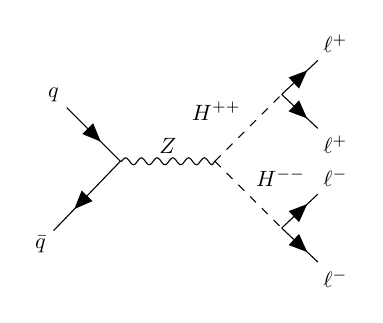
\begin{tikzpicture}[scale=0.8, transform shape]
    \begin{feynman}
        \vertex (a) {$q$};
        \vertex [below right=of a] (b);
        \vertex [right=of b] (c);
        \vertex [above right=of c] (d);
        \vertex [below right=of c] (e);
        \vertex [right=0.3in of d, above right=0.3in] (f1) {$\ell^+$};
            \vertex [right=0.3in of d, below right=0.3in] (f2) {$\ell^+$};
            \vertex [right=0.3in of e, above right=0.3in] (f3) {$\ell^-$};
            \vertex [right=0.3in of e, below right=0.3in] (f4) {$\ell^-$};
        \vertex [below left=of b] (a2) {$\bar{q}$};
        
        \diagram* {
            (a) -- [fermion] (b),
            (a2) -- [anti fermion] (b),
            (b) -- [boson, edge label=$Z$] (c),
            (c) -- [scalar, dashed, edge label=$H^{++}$] (d),
            (c) -- [scalar, dashed, edge label=$H^{--}$] (e),
            (d) -- [fermion] (f1),
            (d) -- [fermion] (f2),
            (e) -- [fermion] (f3),
            (e) -- [fermion] (f4),
        };
    \end{feynman}
\end{tikzpicture}
    \end{center}
\end{itemize}
\end{frame}

\begin{frame}
\frametitle{Introduction}
We attempt to find the mass of the doubly charged Higgs boson, $H^{\pm\pm}$, by analyzing the invariant mass of resultant leptons.\\

\begin{itemize}
    \item<1-> Prior to analysis, simulated events were generated.
    \item<1-> With the data, we calculated the invariant mass for same-charge lepton pairs.
    \item<2-> We then plotted the invariant mass distribution on a histogram.
    \item<3-> Finally, we found the peaks and fitted the distributions with a Gaussian function to attempt to find the mass of $H^{\pm\pm}$.
\end{itemize}
\end{frame}

\section{Methods}
\begin{frame}
\frametitle{Overview}
\begin{itemize}
    \item<1-> We can calculate the invariant mass of a pair of same-charge leptons using the formulas $M=\sqrt{2p_{T_1}p_{T_2}(\cosh(\eta_1-\eta_2)-\cos(\phi_1-\phi_2))}$.
    \item<2-> We define an event, $e_n=\{l_1,\dots,l_n\}$, to be the set of leptons from one collision. We have 1000 events, with $[2,5]$    leptons in each.
    \item<3-> We split the events into 4 groups based on the elements within it.
    \begin{itemize}
        \item<4-> $E_0$: Events with 4 leptons, 2$\ell^+$, and 2$\ell^-$.
        \item<5-> $E_1$: Events with 2 or 3 leptons, such that there are exactly $2\ell^+$ or $2\ell^-$.
        \item<6-> $E_2$: Events with $>2$ $\ell^+$ or $\ell^-$. 
        \item<7-> $E_3$: Any leftover events.
        \item<8-> The groups have no overlapping events, and the union of all groups is the set of all events.
    \end{itemize}
    \item<9-> Define $M(e_n)$, which returns the invariant masses of all same-charge lepton pairs in the event $e_n$.
    \item<10-> For each $e_n\in E_0\cup E_1\cup E_2$, we calculate and save $M(e_n)$.
\end{itemize}
\end{frame}

\subsection{Trial 1}
\begin{frame}
\frametitle{Trial 1 Methods}
\begin{itemize}
\item<1-> Trial 1 considered $E_0$ ($2\ell^+$ and $2\ell^-$).
\item<2-> We consider this the "perfect" trial, because it considers events which are in the ideal, expected form.
\item<3-> For an event $e_n\in E_0$, we can split it into 2 pairs: 1 $\ell^+$ pair and 1 $\ell^-$ pair.
\item<4-> $M(e_n)$, in this case, will return 2 values.
\end{itemize}
\end{frame}

\subsection{Trial 2}
\begin{frame}
\frametitle{Trial 2 Methods}
\begin{itemize}
\item<1-> Trial 2 considered $E_1$.
\item<2-> This is still a good trial, but not "perfect".
\item<3-> For an event $e_n\in E_1$, we can get one pair: either 1 $\ell^+$ pair or 1 $\ell^-$ pair.
\item<4-> $M(e_n)$, in this case, will return 1 value.
\end{itemize}
\end{frame}

\subsection{Trial 3}
\begin{frame}
\frametitle{Trial 3 Methods}
\begin{itemize}
\item<1-> Trial 3 considered $E_2$.
\item<2-> This trial is not as good as the previous two as we have to make assumptions about which lepton pairs to consider.
\item<3-> When there are 3 or more same-charge leptons, we choose 1 pair by choosing the most collimated pair\footnotemark.
\item<4-> $M(e_n)$, in this case, may return 1 or 2 values.
\end{itemize}
\footnotetext[1]{From my research, I found that collimation represented the closeness of two particles. Since we are analyzing two leptons that have decayed from the same $H^{\pm\pm}$, we would expect them to be very collimated.}
\end{frame}

\begin{frame}
\frametitle{Trial 3 Methods - Collimation}
\begin{itemize}
\item<1-> We can find the most collimated pair by iterating over all pairs and minimizing the separation distance.
\item<2-> The separation distance is defined as $\sqrt{(\eta_1-\eta_2)^2+(\phi_1-\phi_2)^2}$.
\end{itemize}
\end{frame}

\section{Code}
\begin{frame}
\frametitle{Codebase}
Analysis with \inline{c++} and graph generation with \inline{matplotlib} in \inline{python}. \\
You may find the code on GitHub: \href{https://github.com/vracton/Doubly-Charged-Higgs-CMS/blob/main/thebeginning/main.cpp}{\inline{\underbar{main.cpp}}} and \href{https://github.com/vracton/Doubly-Charged-Higgs-CMS/blob/main/thebeginning/graph.py}{\inline{\underbar{graph.py}}}.\\
\begin{itemize}
\item<2-> Data was read and sorted into event and element structs.
\item<3-> \inline{elements[]} was sorted by charge with - followed by +.
\item<4-> Every event, $e_n$ was iterated, with its group determined, and invariant mass(es) calculated.
\item<5-> Invariant masses were stored in \inline{results.csv} and brought into \inline{python}.
\item<6-> Graphs were generated with peaks and Guassian functions plotted.
\end{itemize}
\end{frame}

\section{Results}
\begin{frame}
\frametitle{Overview}
\begin{itemize}
\item<1-> We created 5 histograms: Trial 1, Trial 2, Trial 3, Trial 1 \& 2 Combined, and Trial 1, 2, and 3 Combined.
\item<2-> Of the 3017 leptons in total, 2532 (83.9\%) were analyzed.
\end{itemize}
\end{frame}

\subsection{Graphs}
\begin{frame}
\frametitle{Trial 1}
\begin{figure}
    \centering
    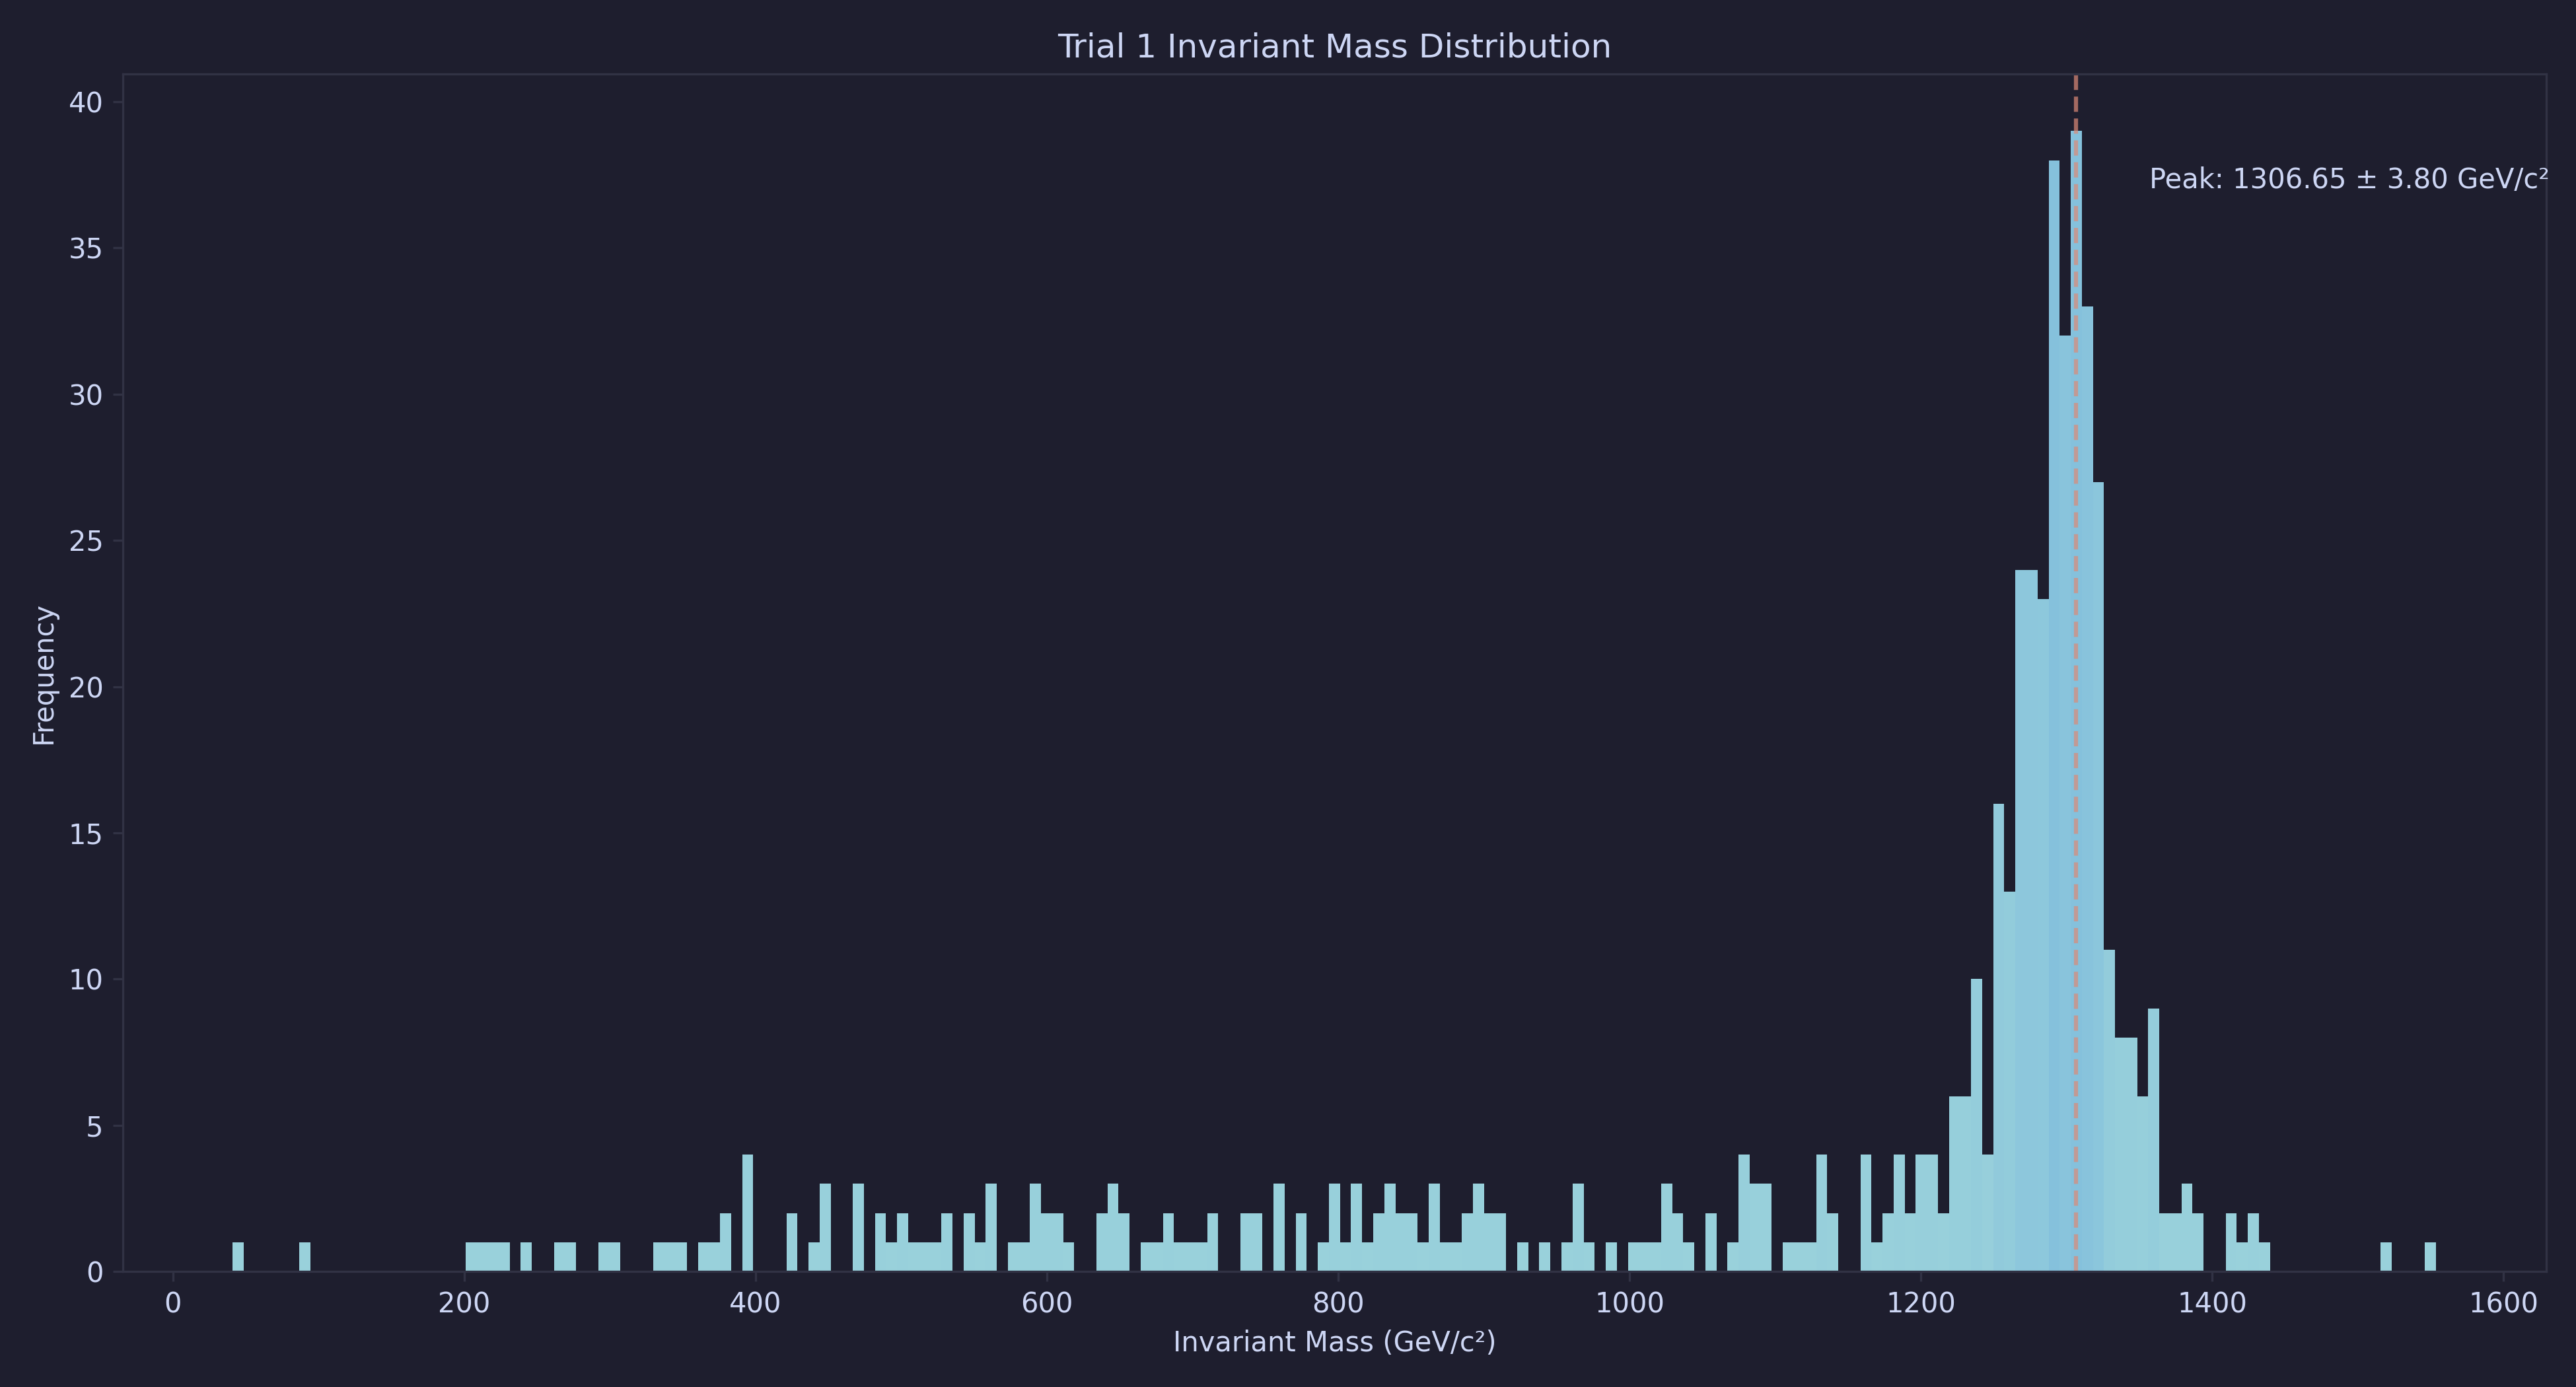
\includegraphics[width=1\textwidth]{dongimages/trial1.png}
    \caption{Histogram of invariant mass distribution for Trial 1}
    \label{fig:trial1}
\end{figure}
\end{frame}

\begin{frame}
\frametitle{Trial 2}
\begin{figure}
    \centering
    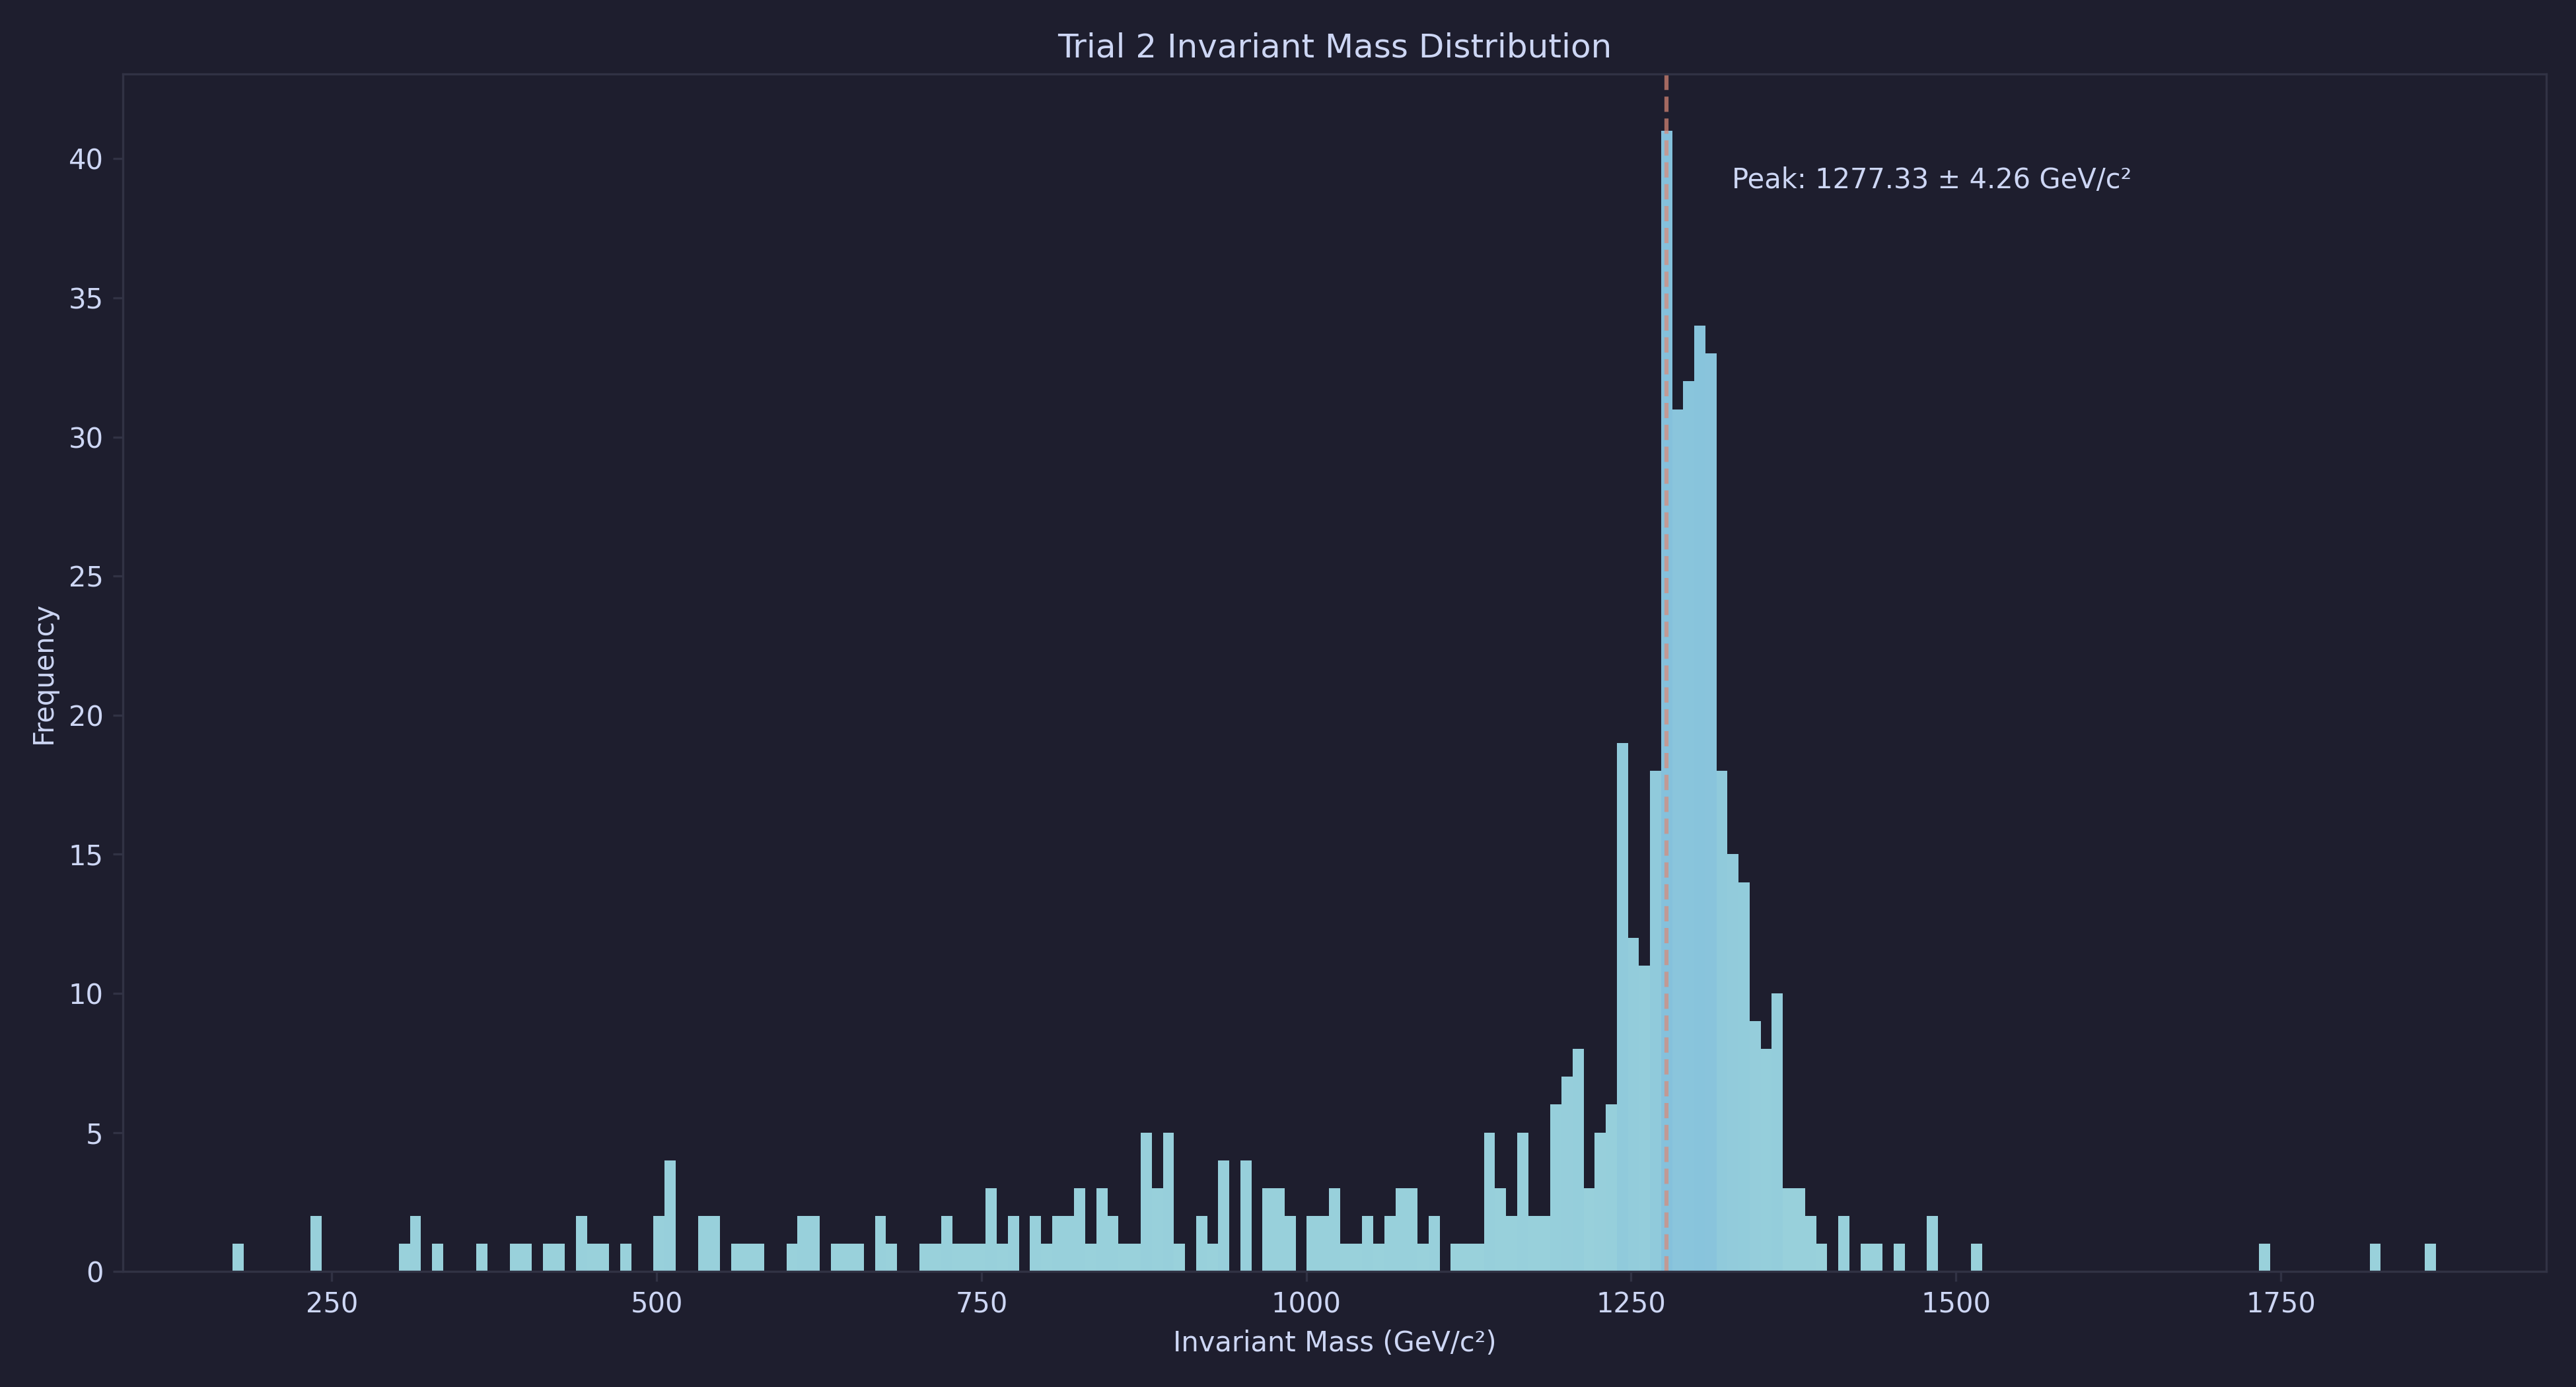
\includegraphics[width=1\textwidth]{dongimages/trial2.png}
    \caption{Histogram of invariant mass distribution for Trial 2}
    \label{fig:trial2}
\end{figure}
\end{frame}

\begin{frame}
\frametitle{Trial 2}
\begin{figure}
    \centering
    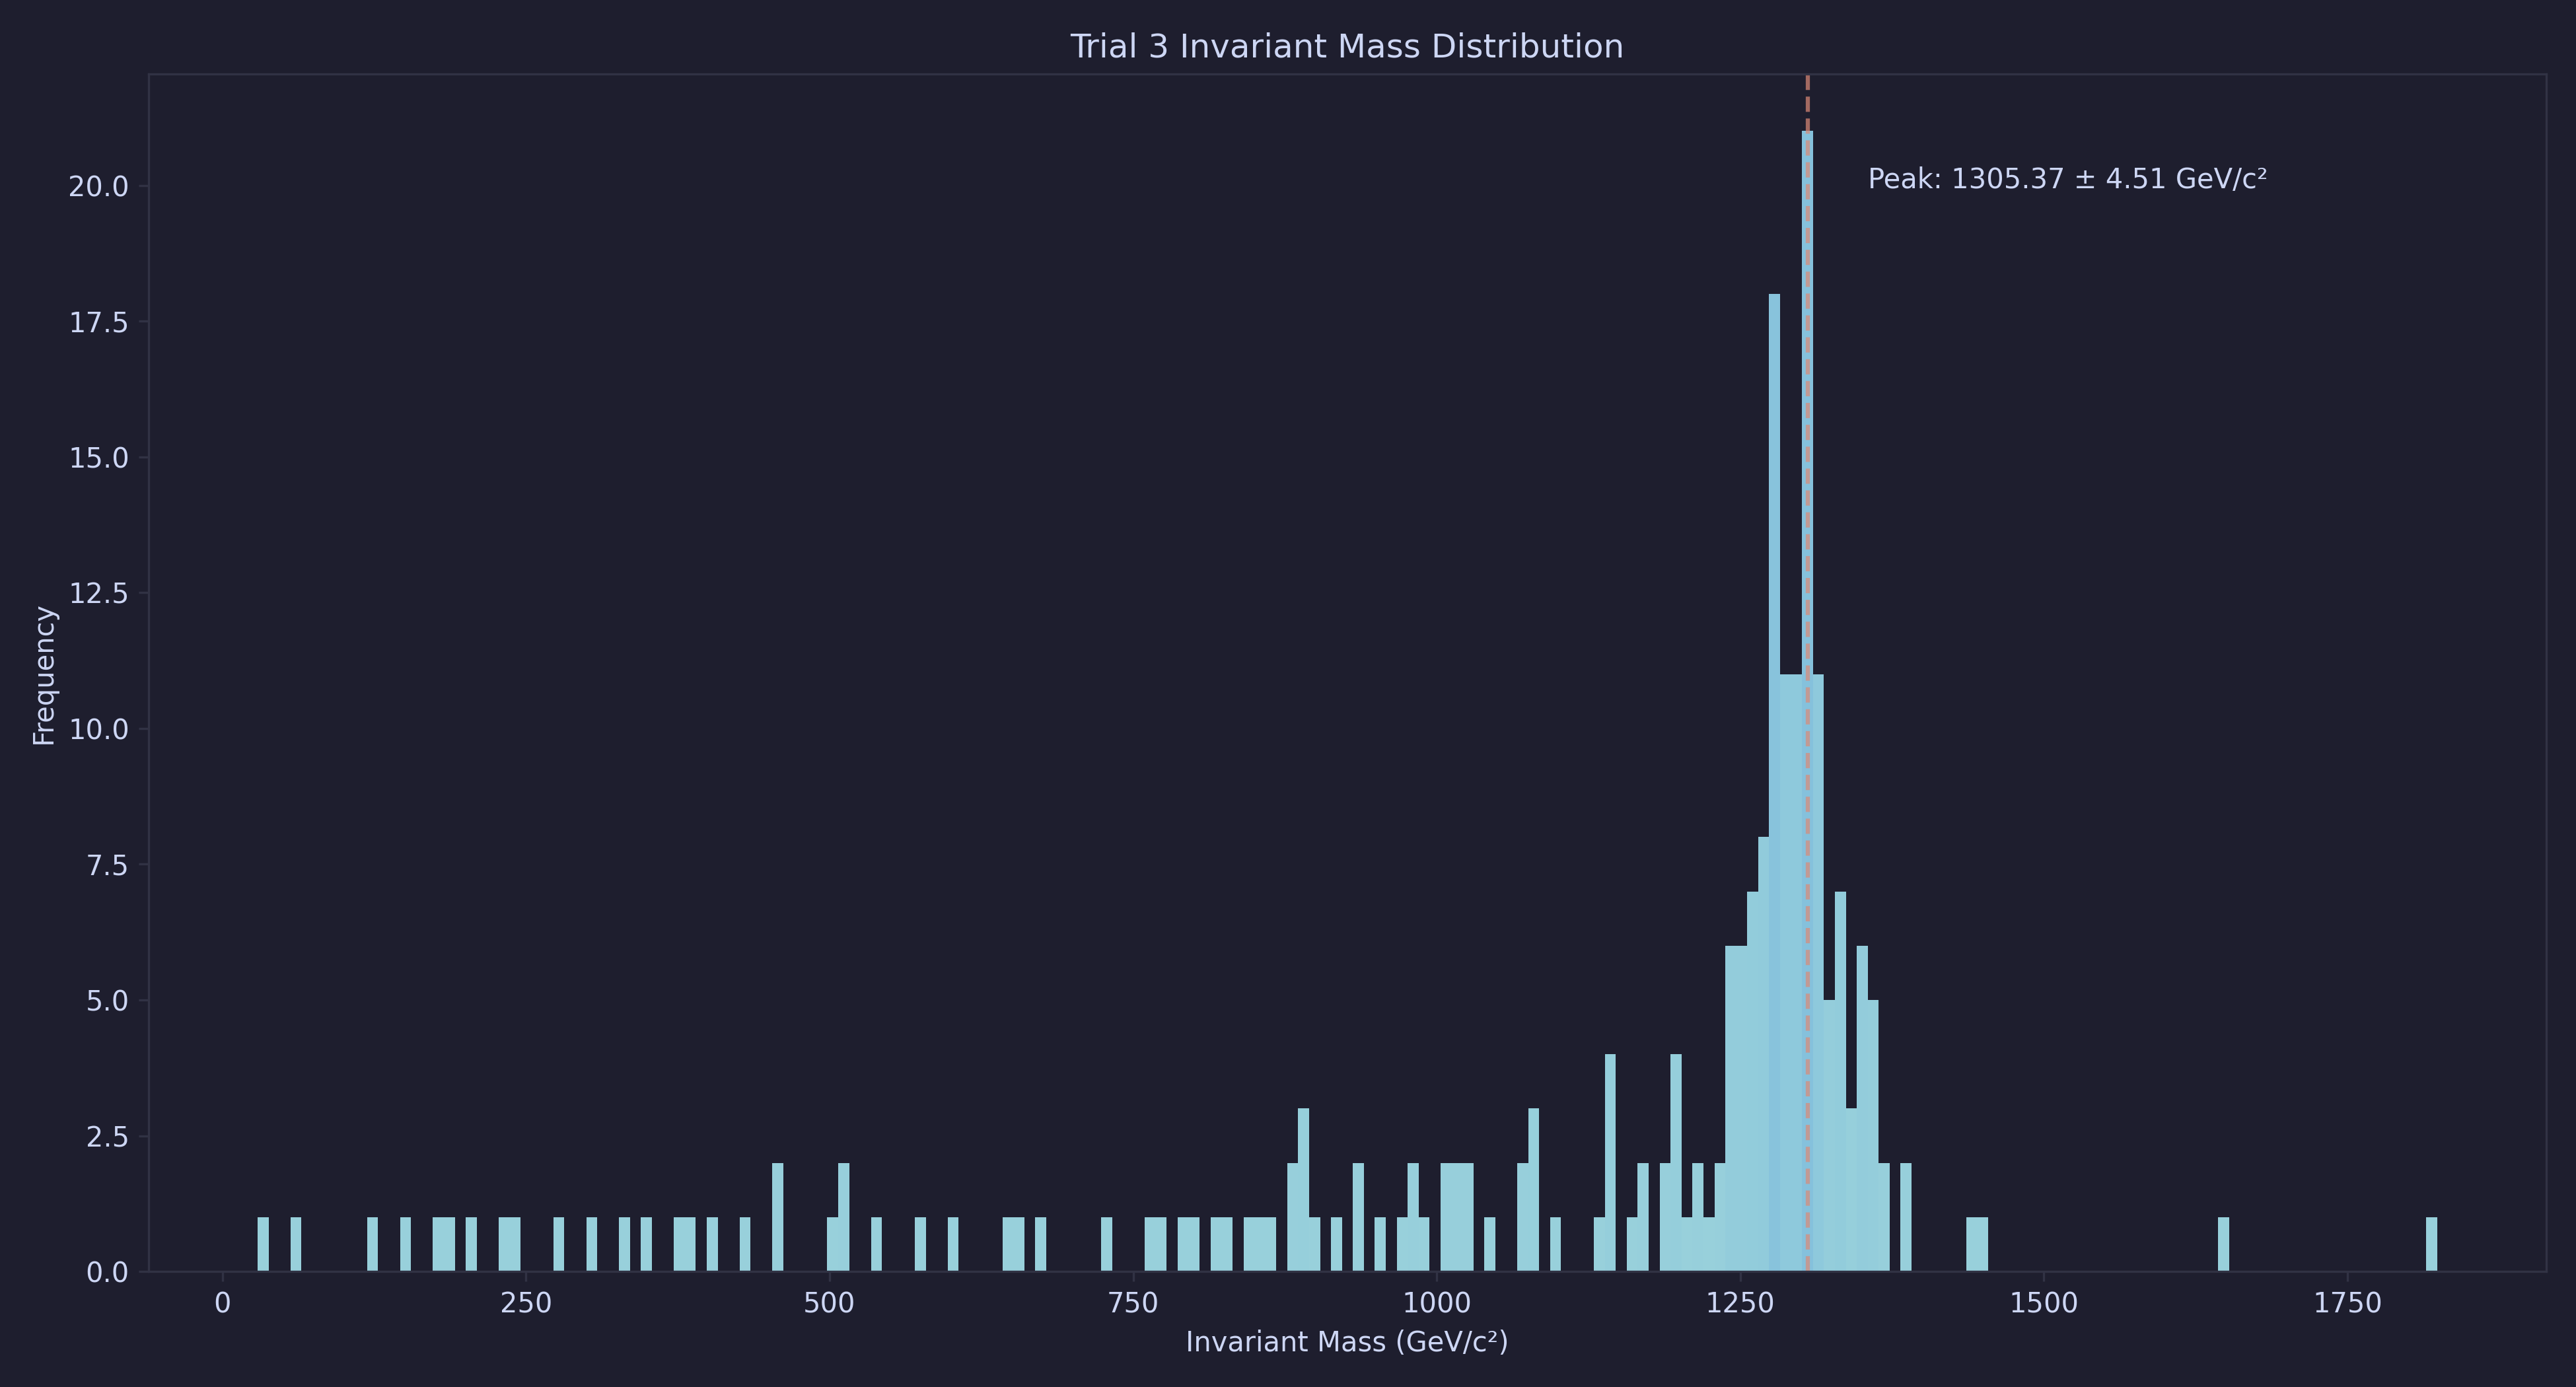
\includegraphics[width=1\textwidth]{dongimages/trial3.png}
    \caption{Histogram of invariant mass distribution for Trial 3}
    \label{fig:trial3}
\end{figure}
\end{frame}

\begin{frame}
\frametitle{Trial 1 \& 2}
\begin{figure}
    \centering
    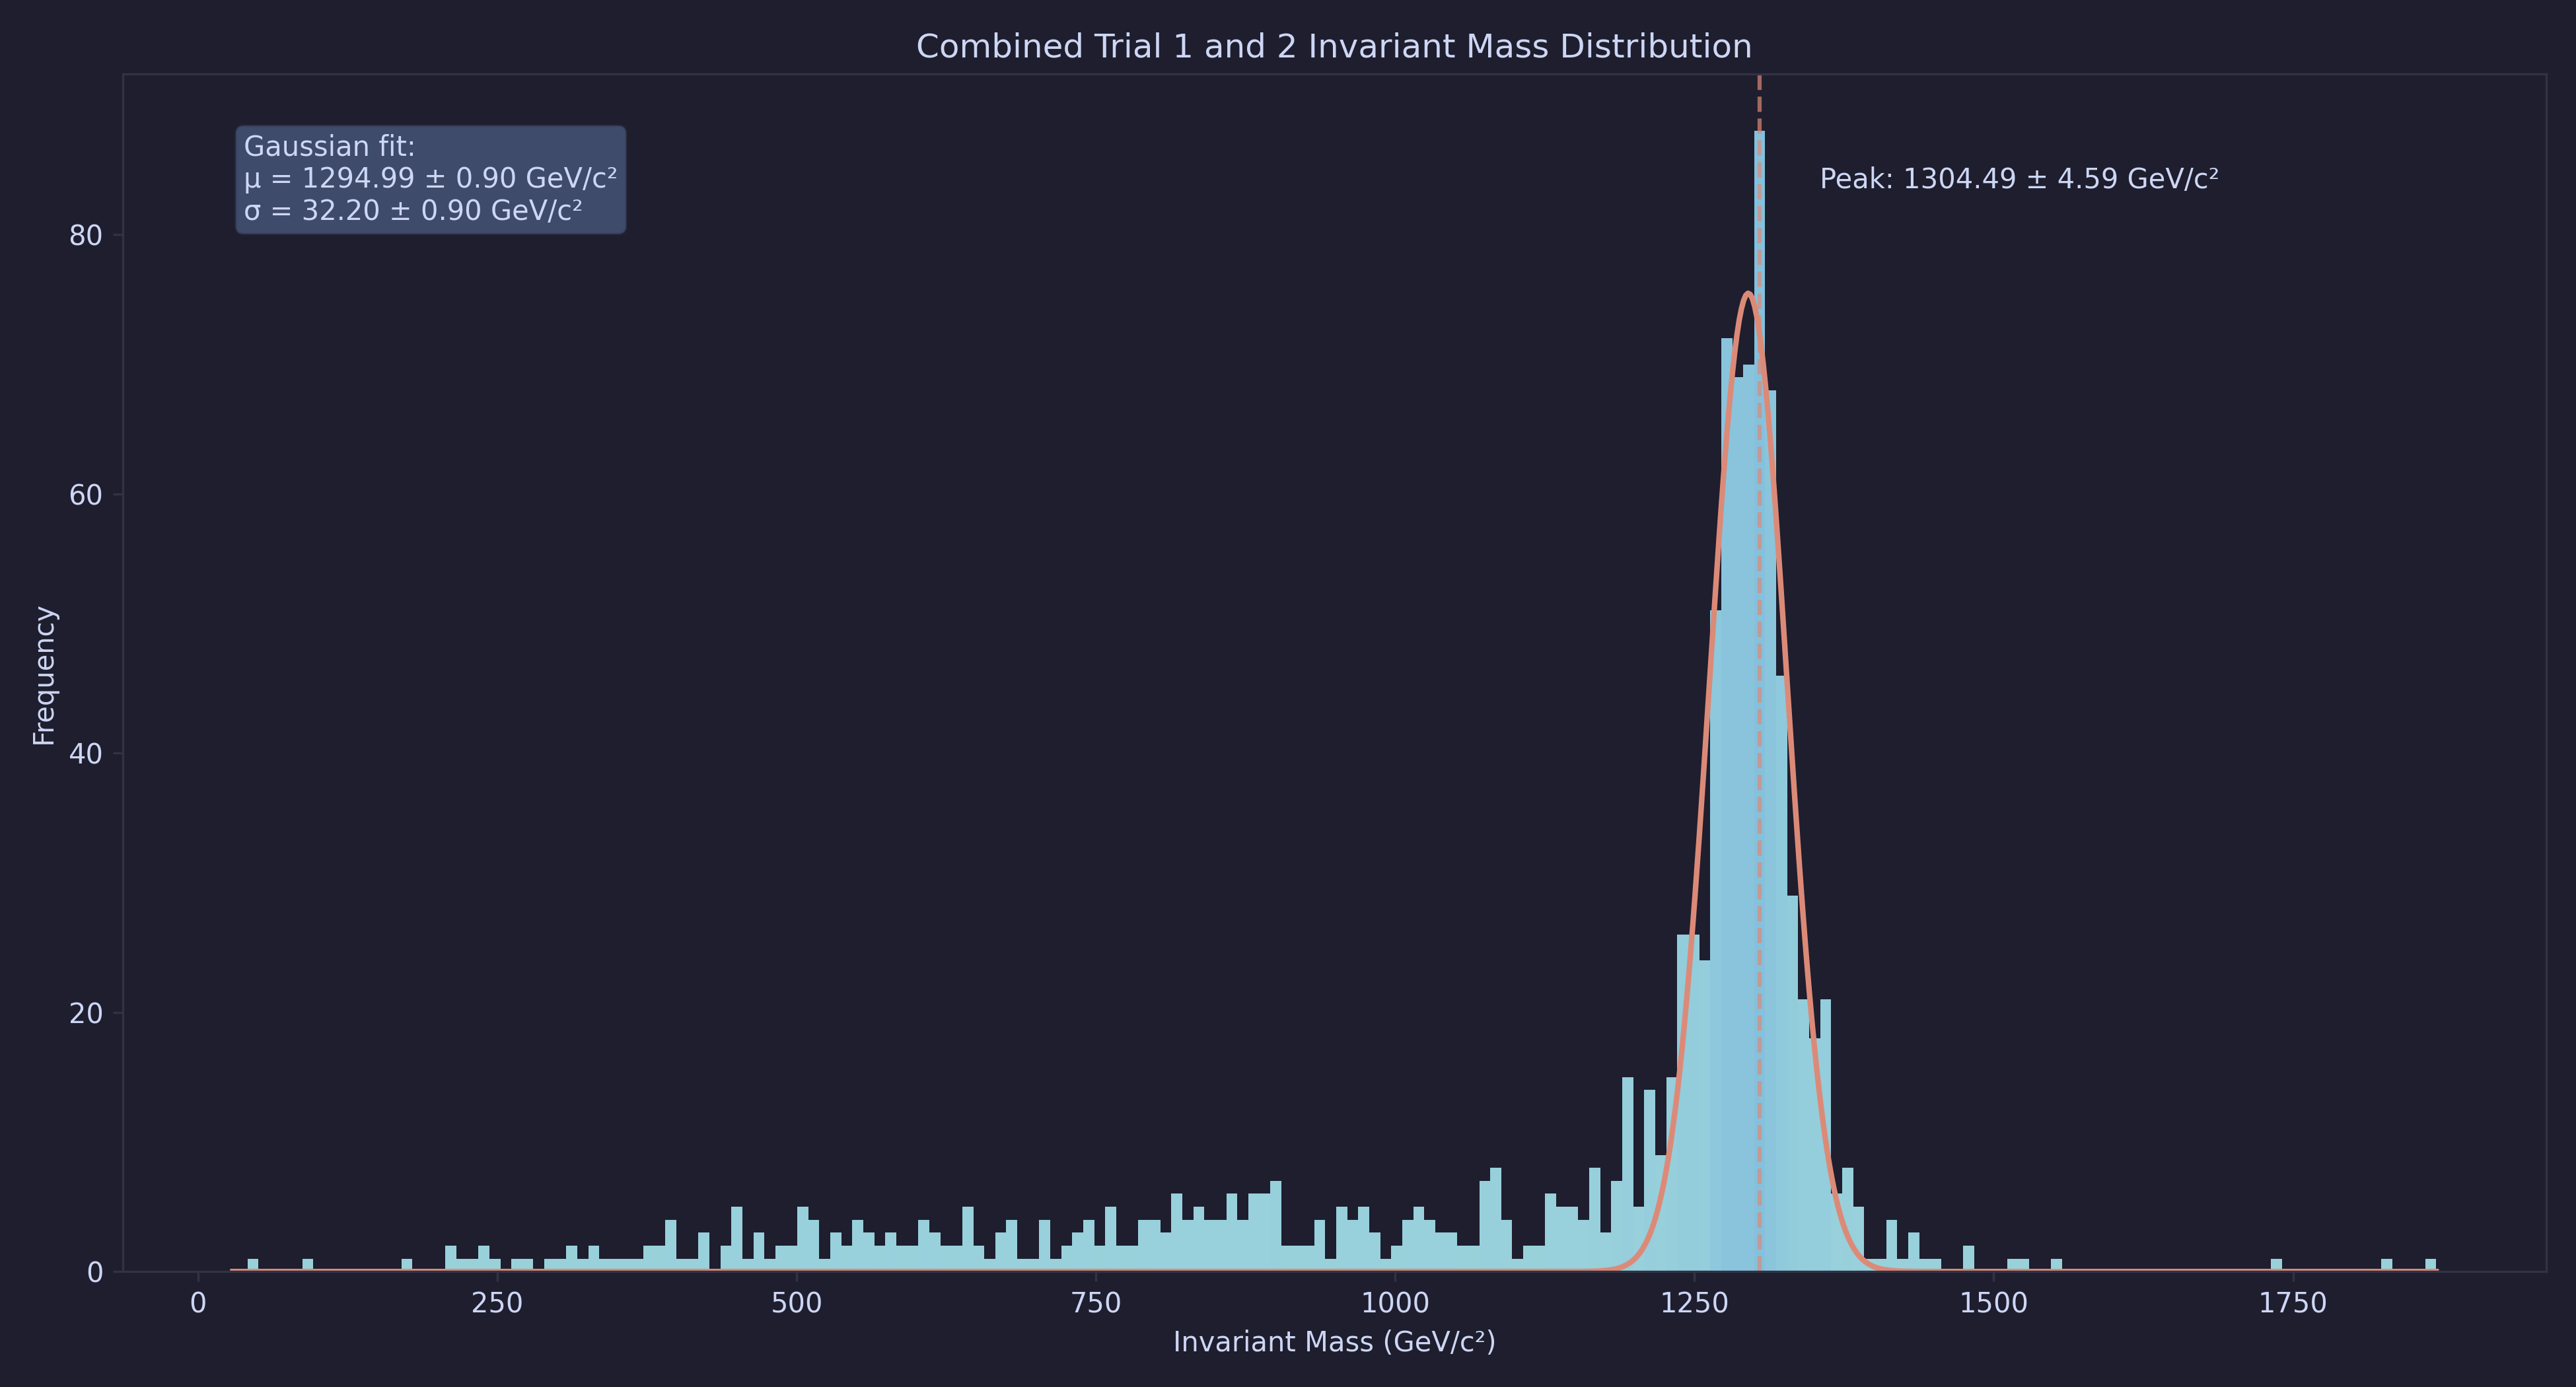
\includegraphics[width=1\textwidth]{dongimages/trial1_2.png}
    \caption{Histogram of invariant mass distribution for Trial 1 \& 2}
    \label{fig:trial1and2}
\end{figure}
\end{frame}

\begin{frame}
\frametitle{Combined}
\begin{figure}
    \centering
    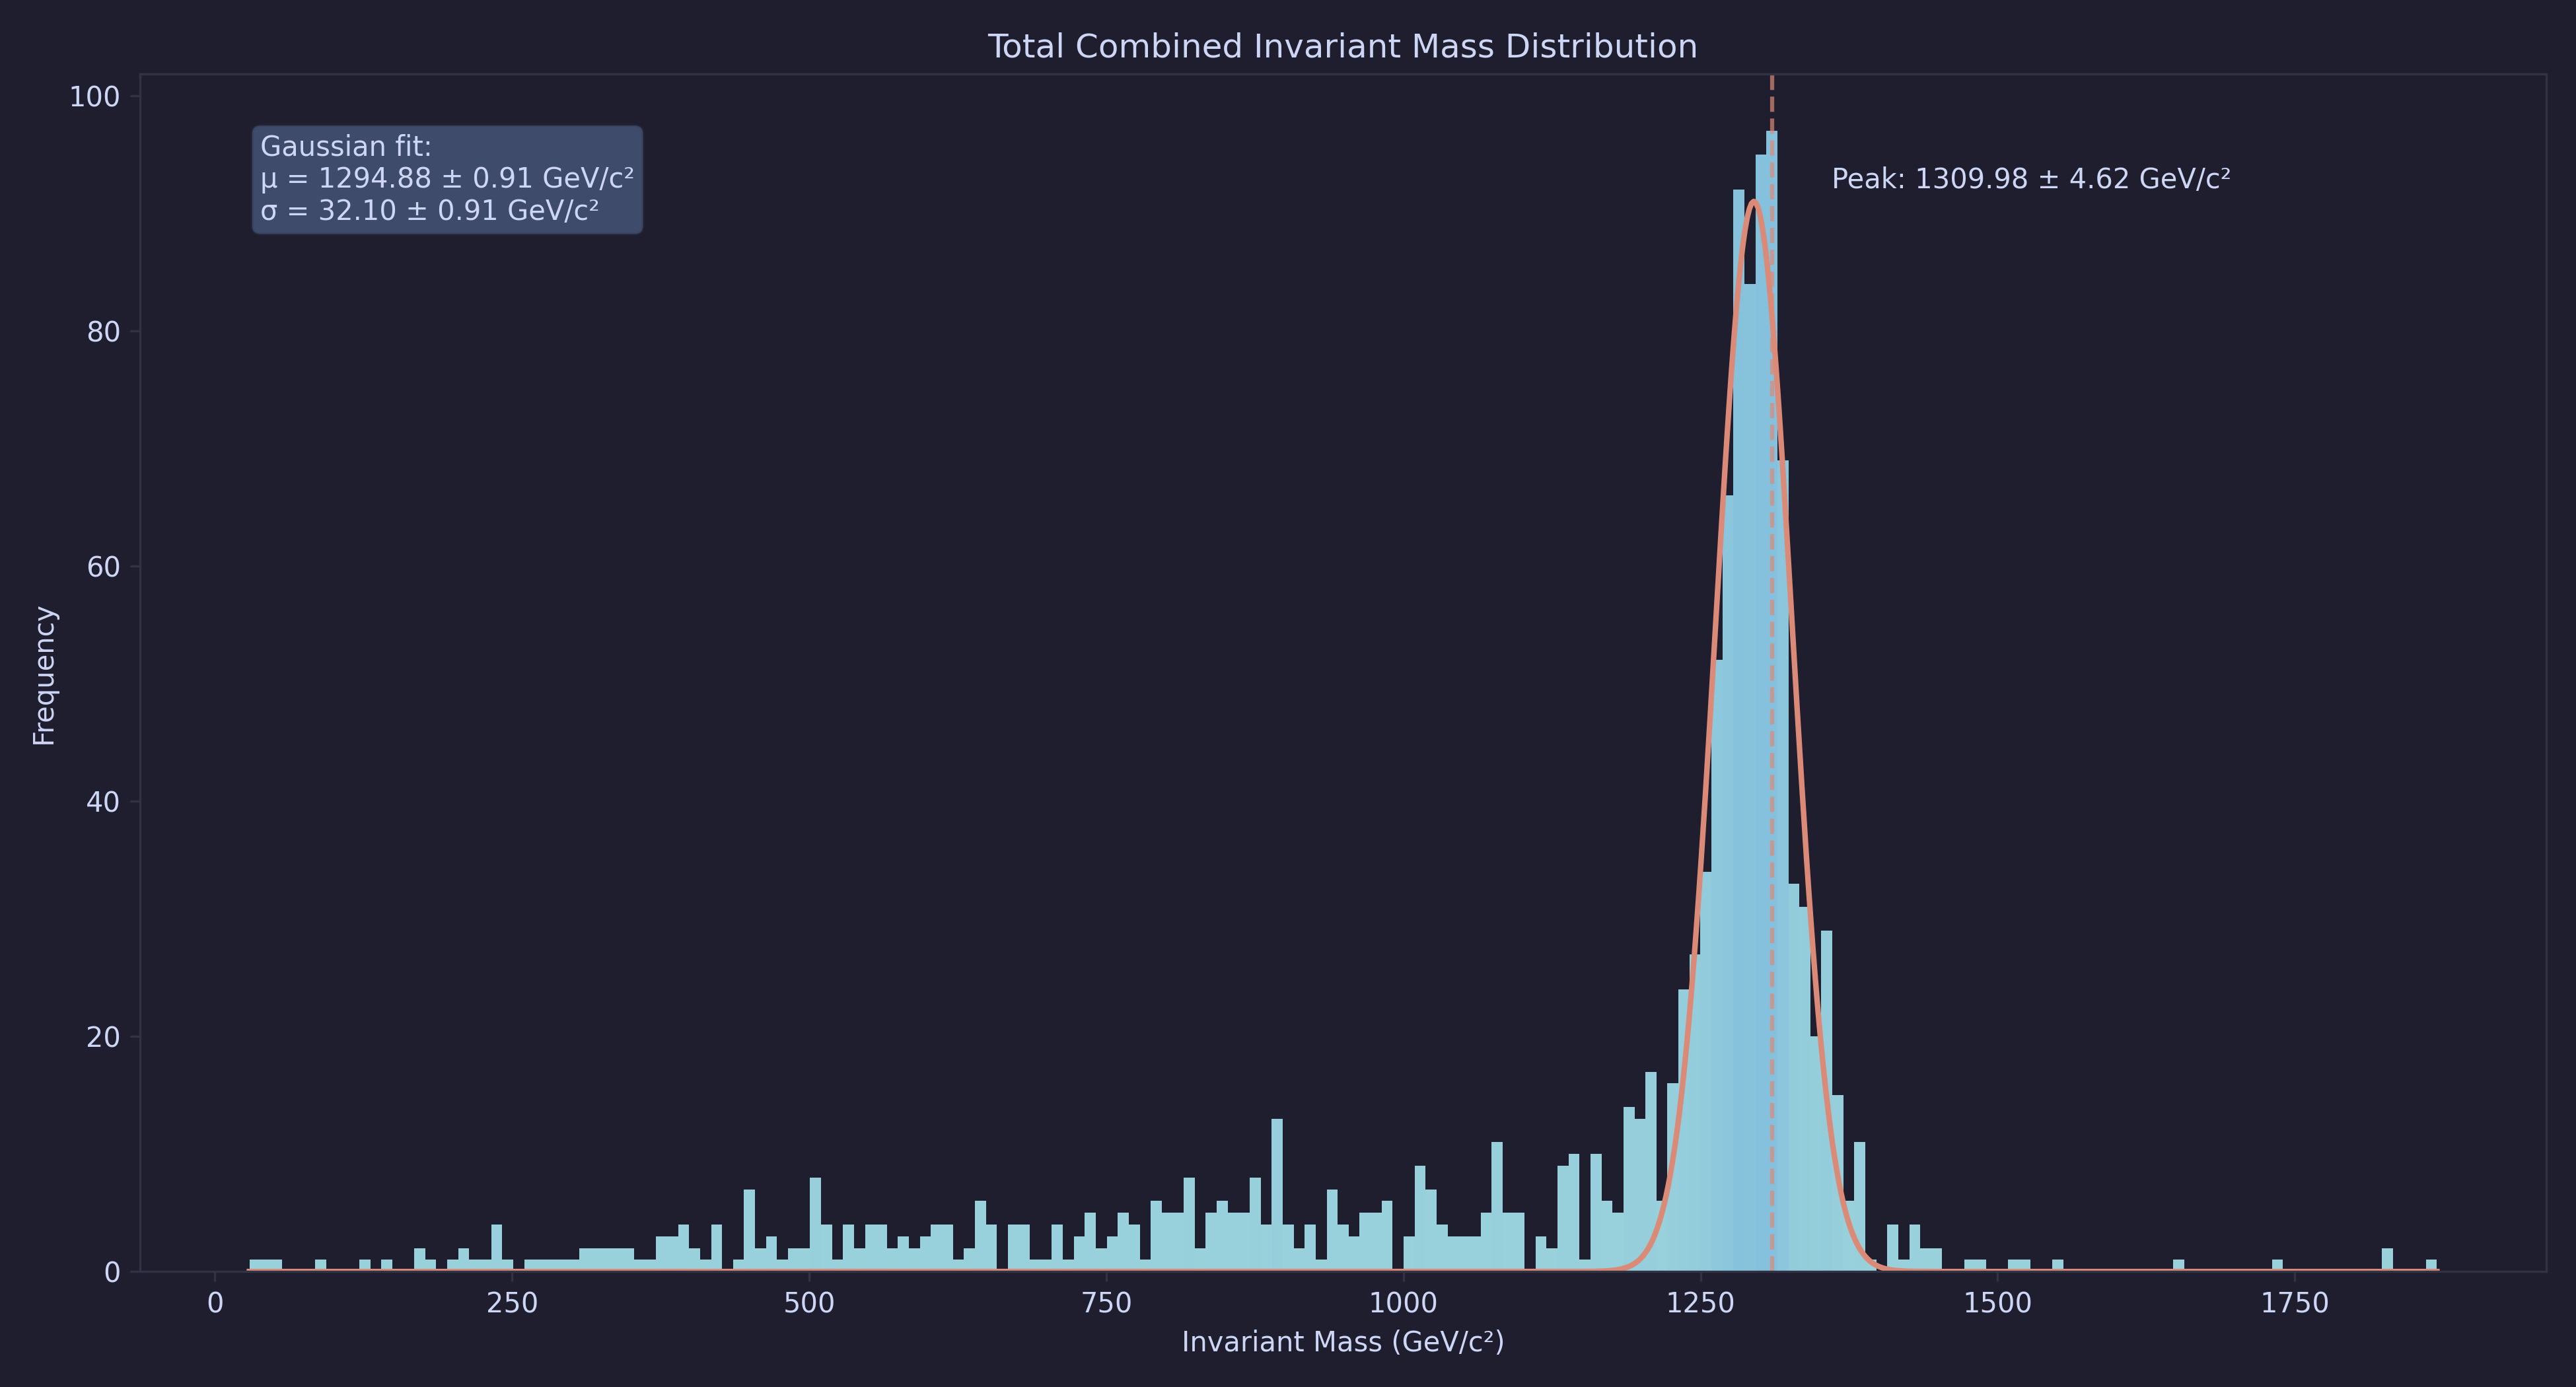
\includegraphics[width=1\textwidth]{dongimages/combined.png}
    \caption{Histogram of invariant mass distribution for Trial 1, 2, and 3}
    \label{fig:trialCombined}
\end{figure}
\end{frame}

\subsection{Conclusion}
\begin{frame}
\frametitle{Conclusion}
\begin{itemize}
    \item<1-> We found the mass of the $H^{\pm\pm}$ to be \underbar{$1294.88\pm0.91$ GeV/c$^2$}.
\end{itemize}
\end{frame}

\begin{frame}
\frametitle{Additional Notes}
\begin{itemize}
    \item<1-> Surprisingly, our results from Trial 3, which we thought would be the worst, was, in fact, more similar to the "perfect" Trial 1 than Trial 2.
    \item<2-> However, in the end, the results of Figure \ref{fig:trial1and2} and Figure \ref{fig:trialCombined} differed by only 0.11 GeV/c$^2$ ($8.5\cdot10^{-3}\%$).
\end{itemize}
\end{frame}

\end{document}